\section{Health Checker}\label{sec:health-checker}
Health Checker je malá služba určená pro správce systému.
Poskytuje informace o tom, zda všechny služby běží, aby správce nebyl nucen přihlašovat se vzdáleně na server a manuálně kontrolovat každou službu.
Výpis stavů jednotlivých služeb je poskytován pomocí jednoduché webové stránky.

\subsection*{Popis algoritmu}
Po nastartování služby je spuštěno REST API na portu 9000 pro komunikaci se správcem.
Jediným endpointem služby je <server:port>/status.
Pokud uživatel pomocí prohlížeče pošle GET požadavek na tuto službu, bude mu vrácen seznam služeb a jejich stavů převedený do formátu JSON (obrázek~\ref{fig:healthchecker_report}).
Stavem aplikace je myšlen status kód a případné chybové hlášky, které služby po zavolání jejich metody <server:port>/ping.

Seznam služeb, které má Health Checker kontrolovat, je načítán z konfiguračního souboru při startu služby.
Jednotlivé služby jsou v seznamu identifikovány na základě IP adresy a portu.

Algoritmus funguje na základě plánovače úloh neboli scheduleru, který jednou do minuty spustí kontrolu všech služeb a jejich stavy uloží do seznamu odkud jsou pak načítány při požadavku na API.
Kontrola se provádí právě posláním HTTP požadavku na <server:port>/ping každé služby a následným uložením odpovědi.

Tento modul umí poskytovat základní informace o aktuálním stavu služeb sytému Coopmaster.
Pokud by se v budoucnu objevil požadavek na historická data, bylo by velmi jednoduché integrovat tuto komponentu s některou z open source platforem určenou pro analytiku a vizualizaci dat.
Například Grafana~\cite{grafana} umožňuje uživatelům vytvářet interaktivní a dynamické panely (dashboardy), které vizualizují různorodé časové řady dat získané z různých zdrojů (obrázek~\ref{fig:health-checker-grafana-dashboard}).


\begin{figure}[H]
    \centering
    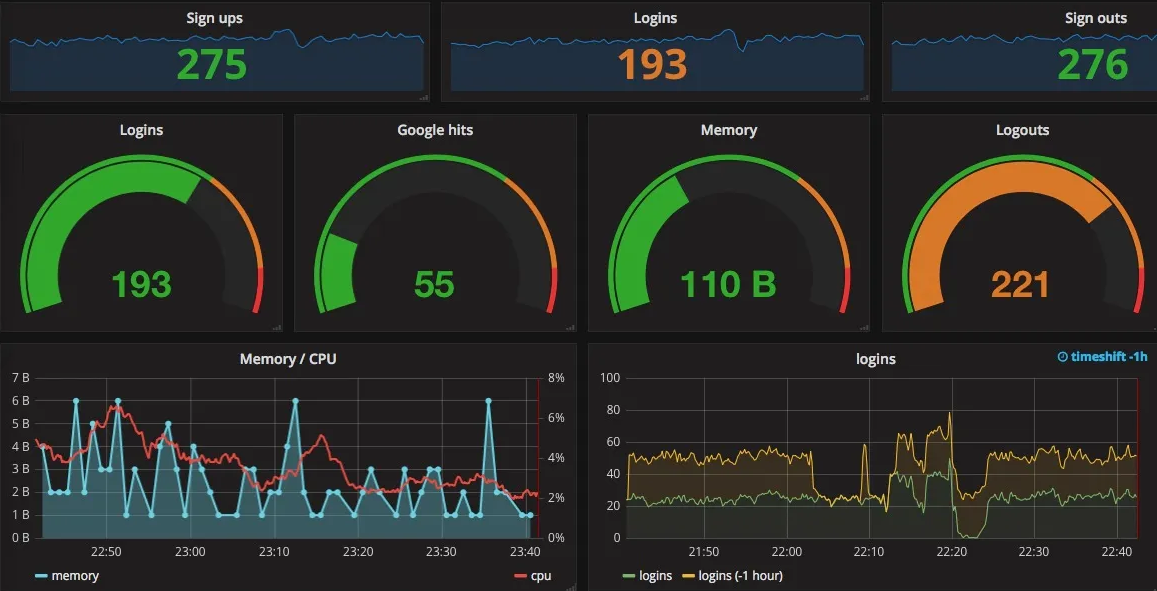
\includegraphics[width=0.8\textwidth]{img/health-checker-grafana-dashboard}
    \captionAuthorSource{Možná vizualizace pomoci platformy Grafana}
    \label{fig:health-checker-grafana-dashboard}
\end{figure}
\begin{figure}[H]
    \centering
    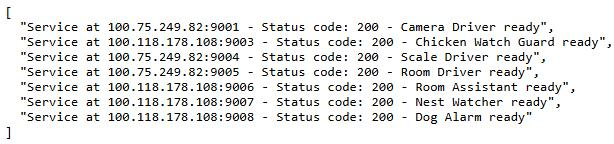
\includegraphics[width=0.8\textwidth]{img/healthchecker_report}
    \captionAuthorSource{Výstup ze služby Health Checker}
    \label{fig:healthchecker_report}
\end{figure}